\documentclass{thesis}
\usepackage{float}
\usepackage{caption}
\usepackage{subcaption}
\usepackage{amsmath}
\begin{document}

\chapter*{Josephson Junctions Through\\
        the RCSJ Model\\
        \normalsize \textit{Spandan Anupam}}

At zero voltage, B. D. Josephson predicted that a supercurrent passing through a junction (called a Josephson junction (JJ)) oscillates with the phase difference as:
\begin{equation}
    I_S = I_C \sin(\phi)
\end{equation}

Where $\phi$ gives the phase difference between the superconducting \textit{banks}. The construction of a josephson junction is quite simple from an outsider's perspective, not as simple from a device manufacturing standpoint.

The device consists of two superconducting banks separated by a non superconducting (mostly insulating) barrier. We get a phase difference with the Ginzburg-Landau (GL) wavefunction travelling in the separate banks, which we called $\phi$ earlier. It does not stop here, it was predicted further that if a constant voltage difference were to be maintained across the junction, it would make the $\phi$ evolve as:
\begin{equation}
    \frac{d\phi}{dt} = \frac{2eV}{\hbar}
\end{equation}

The non superconducting material is called a \textit{weak link}, which can have its own properties along with the junction, which is leading to cutting edge research as I write this. Essentially, what is happening here is that the weak link is allowing Cooper pairs to flow through (called  superconducting \textit{proximitization}) after a certain temperature below the superconducting transition temperature (T$_C$). Coherence lengths vary wildly according to the properties of the material itself, and pose challenges to the experimental side of things in the real world. I have picked a Fig. \ref{planar} from M. Tinkham's tremendous work in superconductivity education, which should bring into picture what kind of a geometry we are talking about in the real world.  It is important to note that this planar geometry isn't the only one, there are many more geometries that people do their measurements in.

\begin{figure}[H]
    \centering
    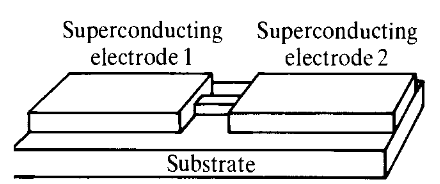
\includegraphics[width=0.4\textwidth]{images/junction_tinkham.png}
    \caption{Planar josephson junction geometry}
    \label{planar}
\end{figure}

As an aside: From here on, we will be considering a gauge invariant phase difference $\gamma$, which will act as a drop in replacement for all $\phi$s in our equations. We have:
\begin{equation}
    \gamma \equiv \phi - (2\pi / \phi_0) \int A.ds 
\end{equation}

The body of work done by Josephson and the equations we write using the one dimensional GL equation is mostly theoretical, and does not apply to the real world where we have many more things going rather than a simple sinusoidal variation. The most common ways to describe a real world junction is either using a Resistively and Capacitively Shunted Junction (RCSJ), or a Tilted Washboard model. Both give out the same equation in their final stage, so we will be focussing on just one of them, the RCSJ model. The RCSJ model models the real world junction by shunting the ideal JJ with a resistor and a capacitor. The resistance accounts for the non zero dissipation in the circuit at a finite voltage and the capacitance accounts for the capacitance between the two superconducting banks.

\section{The Model}
When biasing the junction with current, we write the time dependent phase equation for the RCSJ model as follows:
\begin{equation}
    I = I_C \sin\gamma + V/R + C dV/dt
    \label{rcsj1}
\end{equation}
Using the phase-voltage relation that we defined earlier through the second Josephson relation, the final relation will come out to be:
\begin{equation}
    d^2\gamma /d\tau^2 + Q^{-1} d\gamma /d\tau + \sin \gamma = I/I_C
    \label{rcsj}
\end{equation}
While writing the second order differential equation, we introduce $\tau = \omega_p t$, with $\omega_p$ being called the plasma frequency of the josephson junction, defined as:
\begin{equation}
    \omega_p = (2eI_C/\hbar C)^{1/2}
\end{equation}
And the quality factor, $Q$ is defined by:
\begin{equation}
    Q = \omega_p R C
\end{equation}

I note here the dimensions of different quantities. This will help me to average the potential difference over time in a later point of time. We recall that in a RC circuit, the time constant of the circuit is simply given by $RC$, which is the opposite of frequency. Multiplying $RC$ with a frequency component should lead me to the dimensionless quality factor term. The quality factor just so happens to be identical to $\beta_C^{1/2}$, where $\beta_C$ is a widely used damping parameter. Looking at the equation, we can simply tell that variation in $Q$ will lead to different damping states for the equation.

We now resort to dividing the solution of the differential equation into two regimes, one, where $Q$ is huge, and in the other case, where it is tiny. Computationally, it is hard to accomodate numbers hitting the floating point precision, so it helps to have distinctions and approximations built into our model wherever we can.

For both the cases, the lossless DC regime of the junction is uncoupled from the resistance of the junction. The resistance simply is in parallel and contributes some extra voltage drop across the junction. So whenever I am talking about the potential differences, I will be normalising it by the critical current in the junction and the parallel resistance. Capacitance here, is in between the superconducting banks. In either of Case I and II, I see a pulsating potential drop across the junction and a periodic phase difference between the two banks. I have solved the underdamped equation at $Q=1$ using Runge Kutta methods (and others), and have plotted the potential drop, phase difference across the junction over time ($\tau \propto t$) at a particular value of junction current. The parameters are plotted in Fig. \ref{tauvphi}.

\begin{figure}[H]
    \centering
    \begin{subfigure}[b]{0.48\textwidth}
        \centering
        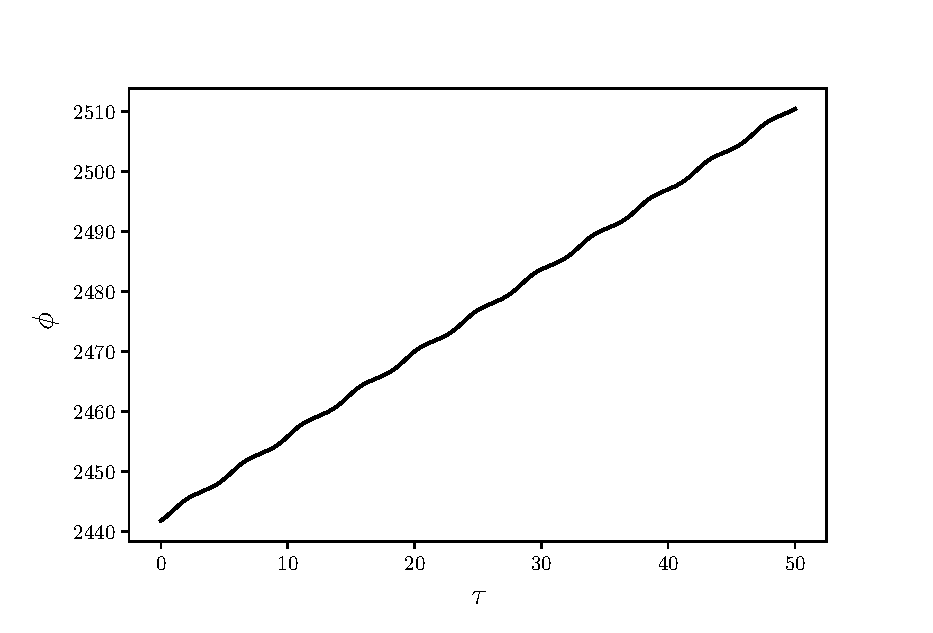
\includegraphics[width=\textwidth]{images/tauphi.eps}
        \caption{Phase change over time}
    \end{subfigure}
    \hfill
    \begin{subfigure}[b]{0.48\textwidth}
        \centering
        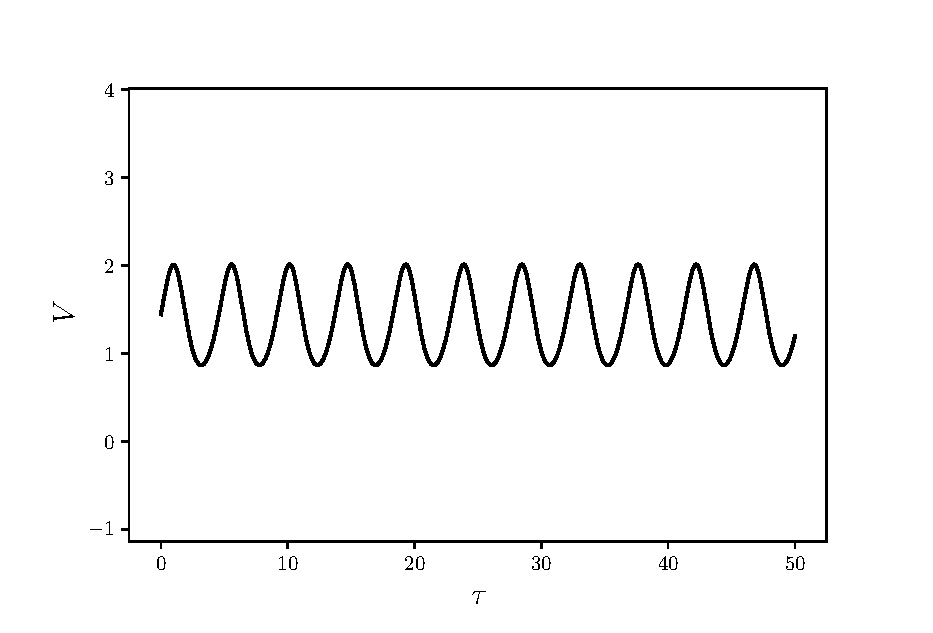
\includegraphics[width=\textwidth]{images/tauV.eps}
        \caption{Potential difference over time}
    \end{subfigure}
    \caption{Plots for I$_C = 1$, at a certain I, in the underdamped case. Voltage oscillations are averaged out to get the DC potential difference across junction.}
    \label{tauvphi}
\end{figure}

\subsubsection{Case I: Underdamped ($Q \ge 1$)}
For large values of C, we will have $Q>1$, in which case, we will have the higher order term in the differential equation, and we will be able to solve it exactly using Equation \ref{rcsj}. This gives out a hysteretic solution, where the scans forward and backward do not give me the same values. When we start increasing $I$, the $V$ stays $0$ till we reach the critical current value, after which it jumps abruptly to a finite voltage. This is what is referred to as the \textit{running state} of the junction. It is in this state that $\gamma$ increases at the rate $2eV/\hbar$. When we come back though, $V$ does not go back to $0$ till a retrapping current $I_r \approx 4I_C/\pi Q$ is reached. This is somewhat expected from a RC circuit, as the circuit can be charged quite easliy without any prior potential difference. While the capacitor is charged, we will have to apply a high negative potential difference across the electrodes to have the capacitor discharge. The equation in focus here is a second order ODE, which we can solve using multiple solvers, but RK4 turns out to be the best.

\begin{figure}[H]
    \centering
    \begin{subfigure}[b]{0.32\textwidth}
        \centering
        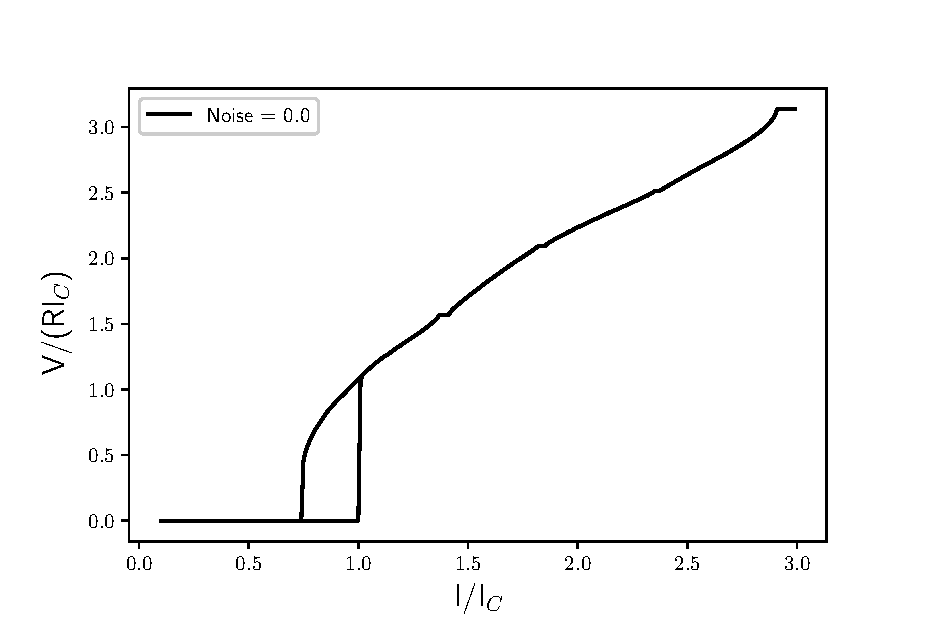
\includegraphics[width=\textwidth]{images/Q_1FE.eps}
        \caption{Forward Euler Solver}
    \end{subfigure}
    \hfill
    \begin{subfigure}[b]{0.32\textwidth}
        \centering
        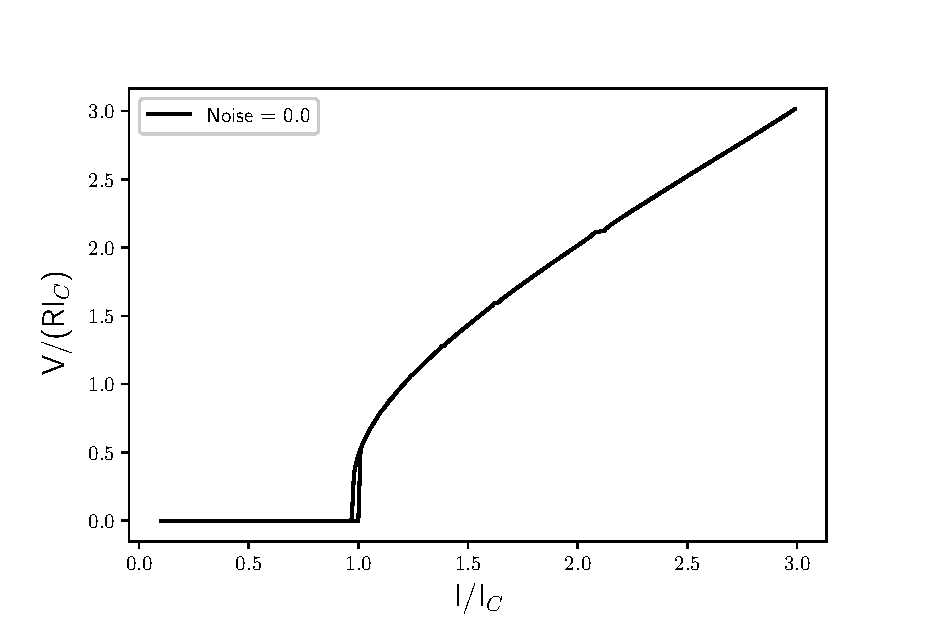
\includegraphics[width=\textwidth]{images/Q_1PC.eps}
        \caption{Predictor Corrector Solver}
    \end{subfigure}
    \hfill
    \begin{subfigure}[b]{0.32\textwidth}
        \centering
        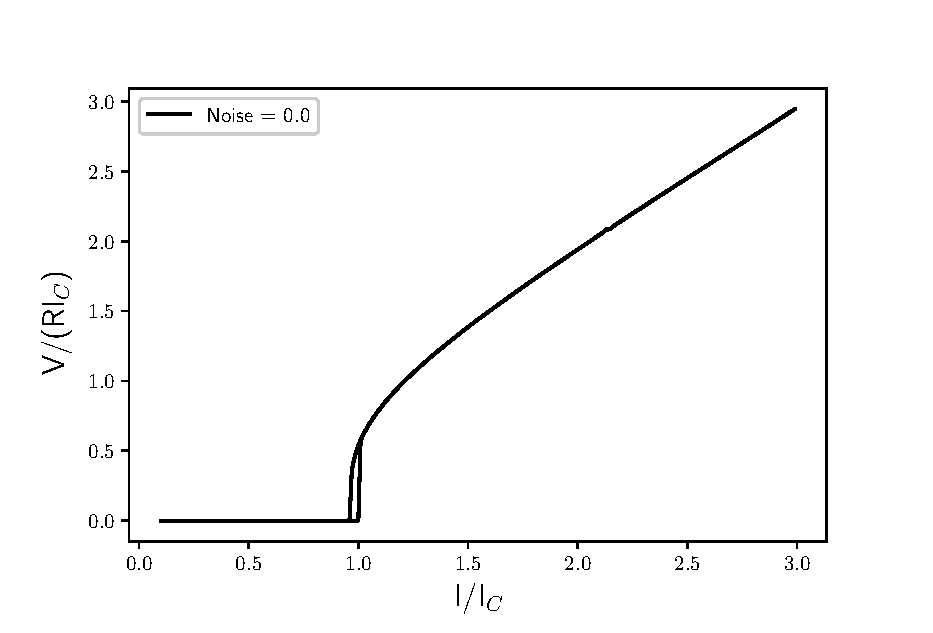
\includegraphics[width=\textwidth]{images/Q_1RK.eps}
        \caption{Runge Kutta (RK4) Solver}
    \end{subfigure}
    \caption{Hysteretic IV curves of the junction in the underdamped condition}
    \label{solvers}
\end{figure}

I have solved the equation using Forward Euler, Predictor corrector and RK4 methods and plotted them in Fig. \ref{solvers}. As expected, the forward Euler method fails miserably in handling the second order equation and gives me a wide hysteresis, which is not ideal in my case. The other two solvers suffice, but RK4 is the best of them as we see.

While I was at it, I wanted to see how the hystersis varied with a change in the capacitance. Plotted in Fig. \ref{Qchange} are the I-V curves for different values of $Q$. Because I have kept the resistance, and the critical current same across the board, the only thing that I am changing effectively is the capacitance ($Q \propto C$).

\begin{figure}[H]
    \centering
    \begin{subfigure}[b]{0.32\textwidth}
        \centering
        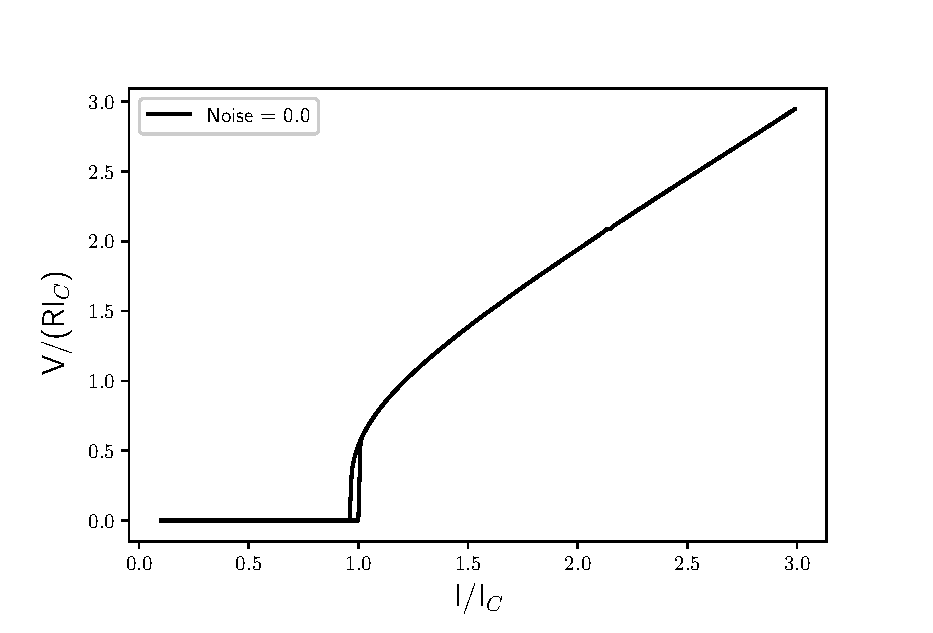
\includegraphics[width=\textwidth]{images/Q_1var.eps}
        \caption{$Q=1$}
    \end{subfigure}
    \hfill
    \begin{subfigure}[b]{0.32\textwidth}
        \centering
        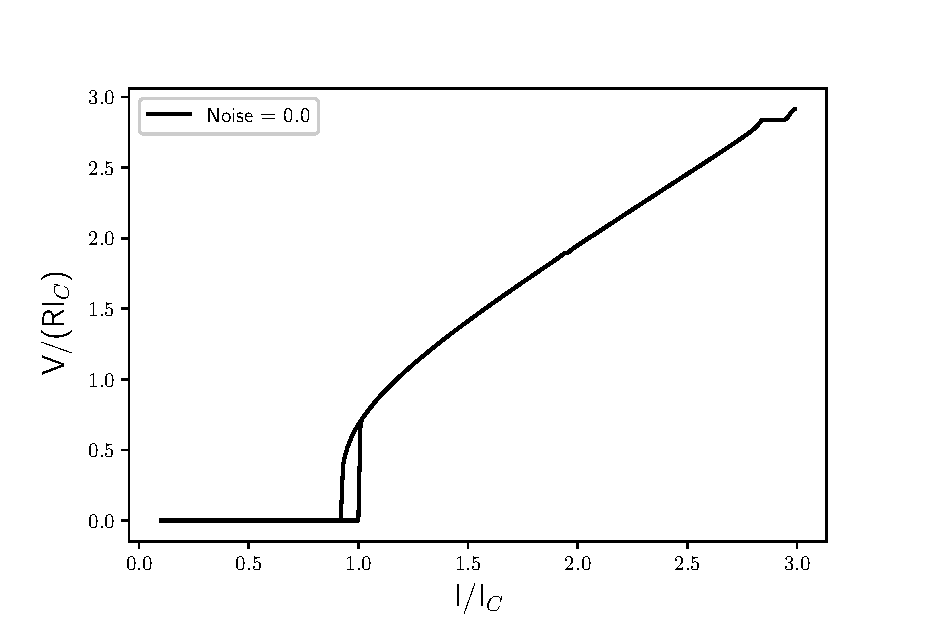
\includegraphics[width=\textwidth]{images/Q_1.1var.eps}
        \caption{$Q=1.1$}
    \end{subfigure}
    \hfill
    \begin{subfigure}[b]{0.32\textwidth}
        \centering
        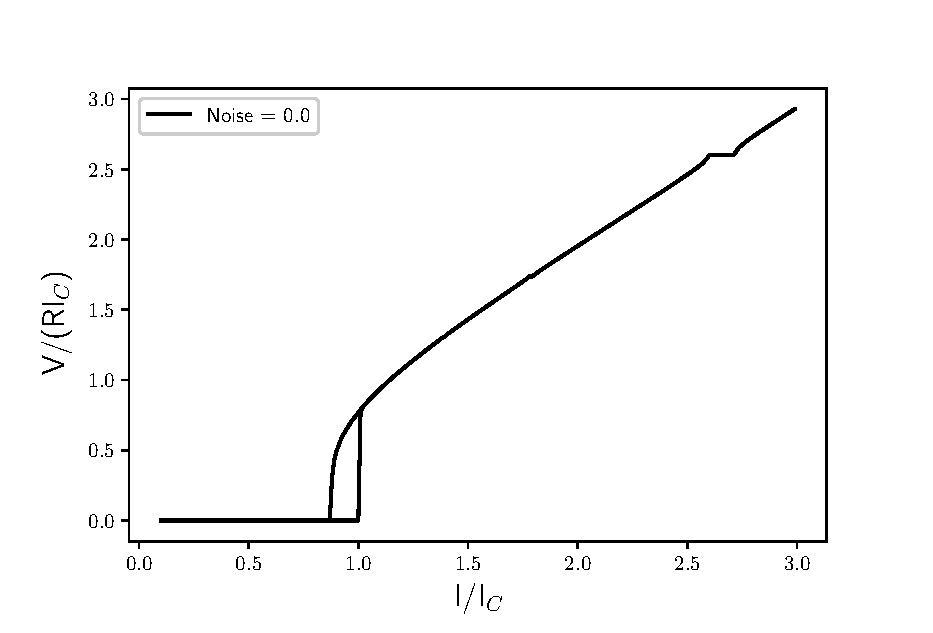
\includegraphics[width=\textwidth]{images/Q_1.2var.eps}
        \caption{$Q=1.2$}
    \end{subfigure}
    \caption{Width of the hysteresis loops changing as I change the quality factor, and essentially the $C$}
    \label{Qchange}
\end{figure}

Again as I expected, the width of the junction changes with the capacitance. The junction is getting charged as we increase the capacitance which might not be what we want in certain cases. To prevent that then, high quality junctions are made with very small dimensions to get rid of the switching nature in them.

\begin{figure}[H]
    \centering
    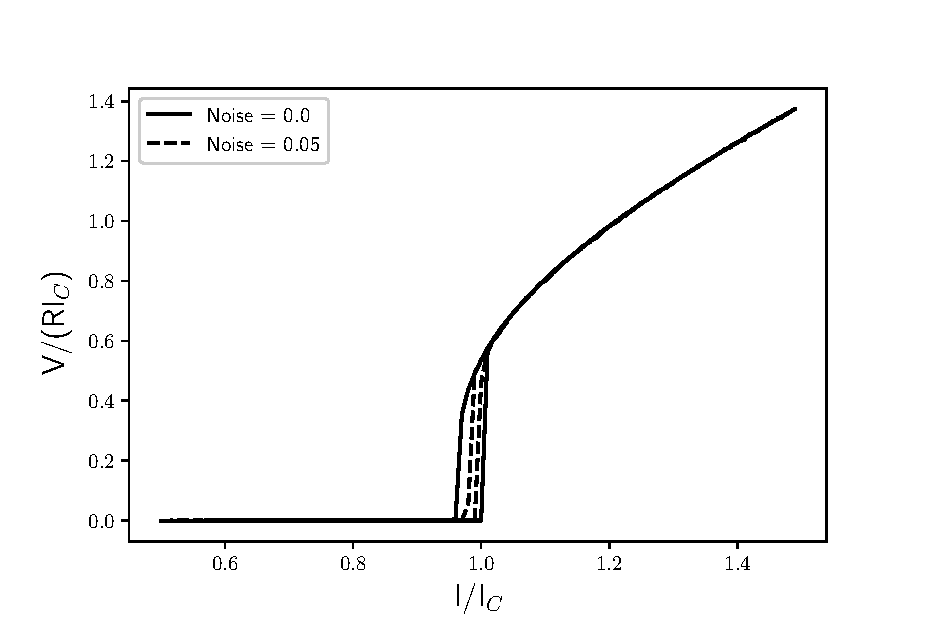
\includegraphics[width=0.5\textwidth]{images/Q_1.eps}
    \caption{Underdamped junction characteristics with and without gaussian white noise}
    \label{noisyunder}
\end{figure}

I note that the calculations carried previously are in the $T=0$ regime, so I assumed no thermal noise. To add an extra level of abstraction to the problem, I went on to add a white gaussian noise to the system. Whith the gaussian noise generator, I am adding a resistance \textit{drive} to Equaiton \ref{rcsj}, with changing $3\sigma$ values. The $\sigma$ here is proportional to thermal noise, which increases as the temperature increases. As I switch on the noise, I see an increase in the retrapping current and a decrease in the critical current. Earlier, particles would have to reach a critical energy (I$_C$) to overcome the barrier. However now, with the help of thermal noise, a particle with a small energy now falls within the range of the barrier without having the exact energy required to scale it. The added drive from the thermal noise helps the particle cross the barrier earlier than before, leading to a decrease in the \textit{actual} critical current. M. Tinkham has referred to this as I$_C$, and the supplied I$_C$ has been called I$_{C0}$. I do not, however make the distinction here, and I understand that the critical current from the junction I-V has decreased. Similar logic can be applied to the retrapping current too, the particle can now apply a higher negative potential difference than it could earlier, and is able to climb down the barrier earlier than before, leading to an increased I$_r$. If I keep increasing the noise, both the characteristic currents collapse into one another and we lose the hysteretic property altogether.

\subsubsection{Case II: Overdamped ($Q\ll 1$)}

Now in the case where we have a small $C$, we are in the overdamped regime. In the limit where $Q \ll 1$, I will be able to ignore the second order term in the differential equation \ref{rcsj}. Doing this leads to a first order differential equation, which makes me lose the hysteretic nature of the curve that I had earlier. Rearranging a few terms in Equation \ref{rcsj}, we land up on:
\begin{align}
    \frac{d\gamma}{dt} &= \frac{2eI_C R}{\hbar} \left( \frac{I}{I_C} - sin \gamma \right)\\
    \implies \frac{d\gamma}{d \tau} &= Q \left( \frac{I}{I_C} - sin \gamma \right)
\end{align}

For $I/I_C > 1$, we will have the slope always positive, and the rate of increase of $\gamma$ will be dependent upon the sign of the $\sin \gamma$. As in the previous case, we will have to average out the voltage over a suitable time period to see anything of value. For both the underdamped and overdamped cases, we see similar solutions for $\gamma$ nad $V$, but different graphs when we plot the $I-V$ curves. A representative plot for the variation of $\gamma$ over $\tau$ has already been given in Fig. \ref{tauvphi}.

The I-V curve of this particlar configuration goes from $V=0$ for $I<I_C$ to Ohm's law at high currents. When the current crosses the critical current, DC voltage is the average of the pulses occuring at a constant frequency $f = 2eV/\hbar$. The IV plot for is given in Fig. \ref{noisyover}. We can see that the particle does not jump to a finite voltage anymore, the transition is smooth, unlike the underdamped condition. Along with the $T=0$ plot, I have plotted the curves that I get a different levels of white noise.

\begin{figure}[H]
    \centering
    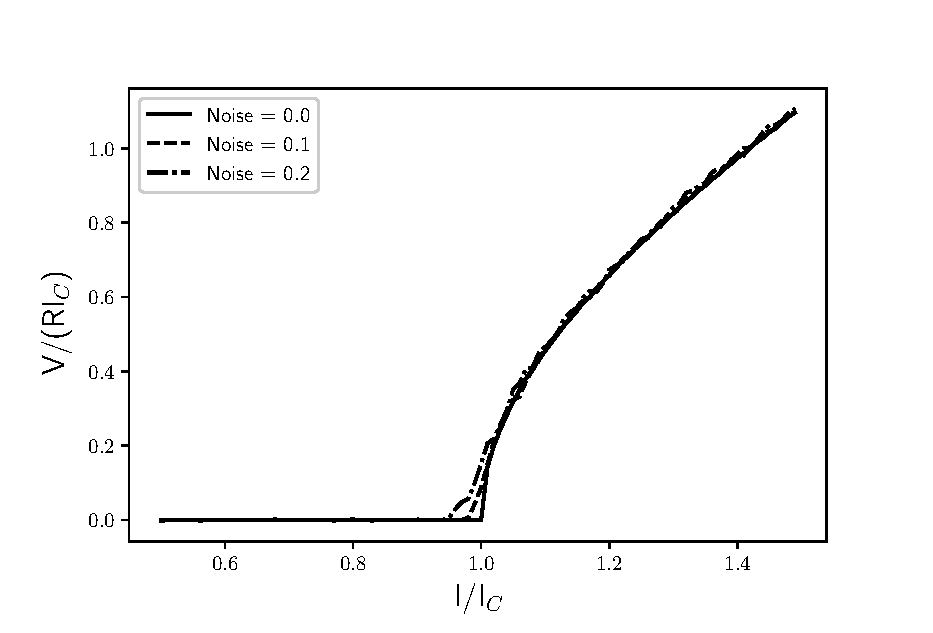
\includegraphics[width=0.5\textwidth]{images/Q_0.001.eps}
    \caption{Overdamped junction with different levels of gaussian white noise added}
    \label{noisyover}
\end{figure}

Ambegaokar and Halperin showed that the resistance never really goes zero as it does for the underdamped case. Instead of making an escape over the barrier, the particle now has a range of current over which it can diffuse through the barrier. In plain terms, the resistance does not go to zero at finite temperatures, and instead stays at a very low value. The exponentially small resistance shows up as \textit{rounding} off of the junction knee as the noise increases. The effect is quite visible in the graph that I compiled, and I would say I have been successful in modelling the effect of noise quite well.

\section{References}
\begin{enumerate}
    \item Tinkham, M., Introduction to Superconductivity 2nd Ed. (1996)
    \item Ambegaokar, V. and Halperin, B. I., Voltage Due to Thermal Noise in the dc Josephson Effect, Phys. Rev. Lett. 22, 1364 (1969).
\end{enumerate}
\end{document}
